%%%%%%%%%%%%%%%%%%%%%%%%%%%%%%%%%%%%%%%%%
% a0poster Landscape Poster
% LaTeX Template
% Version 1.0 (22/06/13)
%
% The a0poster class was created by:
% Gerlinde Kettl and Matthias Weiser (tex@kettl.de)
%
% This template has been downloaded from:
% http://www.LaTeXTemplates.com
%
% License:
% CC BY-NC-SA 3.0 (http://creativecommons.org/licenses/by-nc-sa/3.0/)
%
%%%%%%%%%%%%%%%%%%%%%%%%%%%%%%%%%%%%%%%%%

%-------------------------------------------------------------------------------
%	PACKAGES AND OTHER DOCUMENT CONFIGURATIONS
%-------------------------------------------------------------------------------

\documentclass[a0, landscape]{a0poster}

\usepackage{multicol} % This is so we can have multiple columns of text side-by-side
\columnsep=100pt % This is the amount of white space between the columns in the poster
\columnseprule=3pt % This is the thickness of the black line between the columns in the poster

\usepackage[svgnames]{xcolor} % Specify colors by their 'svgnames', for a full list of all colors available see here: http://www.latextemplates.com/svgnames-colors

%\usepackage{times} % Use the times font
\usepackage{palatino} % Uncomment to use the Palatino font
\usepackage{graphicx} % Required for including images
\graphicspath{{figures/}} % Location of the graphics files
\usepackage{booktabs} % Top and bottom rules for table
\usepackage[font=small,labelfont=bf]{caption} % Required for specifying captions to tables and figures
\usepackage{amsfonts, amsmath, amsthm, amssymb} % For math fonts, symbols and environments
\usepackage{wrapfig} % Allows wrapping text around tables and figures
\usepackage{url}
\begin{document}

%----------------------------------------------------------------------------------------
%	POSTER HEADER
%----------------------------------------------------------------------------------------

% The header is divided into three boxes:
% The first is 55% wide and houses the title, subtitle, names and university/organization
% The second is 25% wide and houses contact information
% The third is 19% wide and houses a logo for your university/organization or a photo of you
% The widths of these boxes can be easily edited to accommodate your content as you see fit

\begin{minipage}[b]{0.9\linewidth}
\veryHuge \color{NavyBlue} \textbf{{\tt MRI2MRI}: A deep convolutional network that accurately transforms between brain MRI contrasts} \color{Black}\\ % Title
%\Huge\textit{An Exploration of Complexity}\\[1cm] % Subtitle
\huge \textbf{Sa Xiao\textsuperscript{1}, Yue Wu\textsuperscript{1}, Aaron Lee\textsuperscript{1}, \& Ariel Rokem\textsuperscript{2}}\\ % Author(s)
\Large 1. The Department of Ophthalmology, The University of Washington \\ 2. The eScience Institute, The University of Washington \\% University/organization
\Large Contact: \texttt{arokem@uw.edu} $|$ Download: \texttt{http://arokem.github.io/2018-ncec-mri2mri-poster/poster.pdf}
\end{minipage}
%
%\begin{minipage}[b]{0.25\linewidth}
%\color{DarkSlateGray}\Large \textbf{Contact Information:}\\
%Department Name\\ % Address
%University Name\\
%123 Broadway, State, Country\\\\
%Phone: +1 (000) 111 1111\\ % Phone number
%Email: \texttt{john@LaTeXTemplates.com}\\ % Email address
%\end{minipage}
%
\begin{minipage}[b]{0.1\linewidth}

\includegraphics[width=10cm]{UWlogo.png}
\end{minipage}

\vspace{0.5cm} % A bit of extra whitespace between the header and poster content

%----------------------------------------------------------------------------------------

\begin{multicols}{3} % This is how many columns your poster will be broken into, a poster with many figures may benefit from less columns whereas a text-heavy poster benefits from more

%----------------------------------------------------------------------------%	Introduction
%----------------------------------------------------------------------------

\section*{Introduction}

MRI creates images that are sensitive to different aspects of the tissue, and
susceptible to different imaging artifacts. The relationships between different
imaging contrasts are nonlinear and spatially- and tissue-dependent
\cite{Vymazal1995-zo}. This poses several difficulties in the interpretation of
multi-modal MRI. For example, analysis that requires accurate registration of
images into the same coordinate frame currently requires the use of algorithms
that can match images with different contrasts \cite{Klein2009-gq}. While this
often works well, these algorithms can be over-sensitive to large, prominent
features, such as edges of the tissue, and are more error-prone when images
have low SNR, or represent very different features. Moreover, a better
understanding of complementary information provided in different contrasts will
allow better characterization of tissue properties.

\rule{\linewidth}{0.4pt}

%----------------------------------------------------------------------------
%	MATERIALS AND METHODS
%----------------------------------------------------------------------------
\normalsize
\section*{Materials and Methods}

We used the IXI dataset (\url{http://brain-development.org/ixi-dataset/}): T1w, T2w, PD, MRA, and DWI (16 directions, at b-value of 1000, one b=0) for N=567 subjects are available. A convolutional neural network was trained to learn the mapping between different MRI images in a training set (n=338).  We used a U-net architecture \cite{Ronneberger2015-ua}, with loss evaluated on “perceptual loss” \cite{Johnson2016-ac}: the activation of the first layer of a pretrained VGG16 network \cite{Simonyan2014-ua}, a  cost function that induces image similarity and prevents over-smoothing. Training used the Adam optimizer (learning rate: 0.0002). The implementation used Pytorch (https://pytorch.org).
A group of participants (n=79), set aside as a test set (not shown to the algorithm during training) was used to evaluate registration. We used a state-of-the-art registration algorithm \cite{Avants2008-sa}, implemented in DIPY \cite{Garyfallidis2014-el} to register DWI b=0 to corresponding T1w images, using a mutual information metric to find the best affine transformation for registration. To simulate participant motion, known rotation and translation were applied to the b=0 image and the T1w was registered to the b=0. For comparison, we also synthesized a T1w-analog from the b=0 image using the DL network and used the synthesized image with the same registration algorithm. Registration errors were calculated relative to known ground truth as mean absolute error (MAE), for translation and rotation components of the registration.

\begin{minipage}[b]{0.5\linewidth}
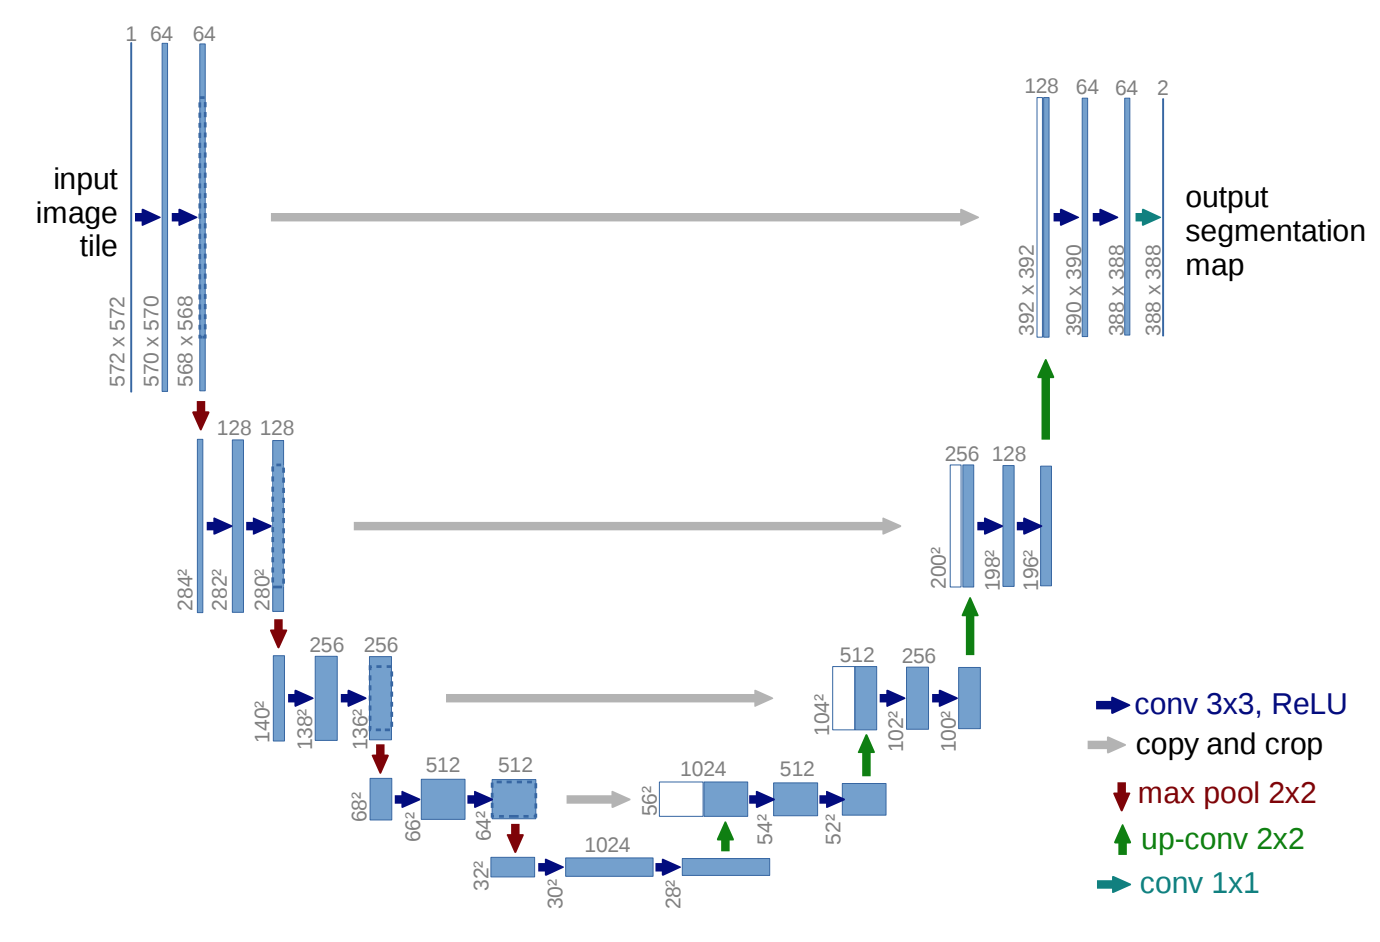
\includegraphics[width=15cm]{unet.png}
\center U-Net architecture
\end{minipage}
\\
\rule{\linewidth}{0.4pt}

\section*{Other applications}

\begin{minipage}[t]{1\linewidth}
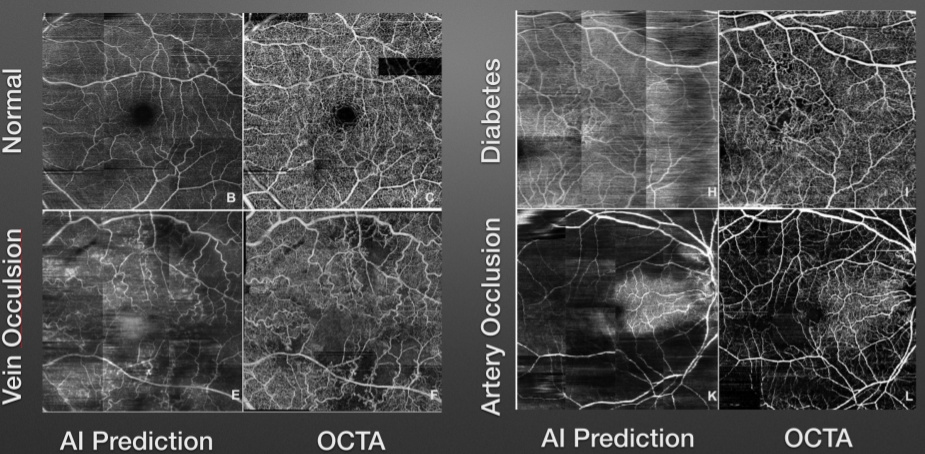
\includegraphics[width=18cm]{octa.png}
\\
AI-synthesized retinal perfusion images in patients with diseases that were not part of the training set.
\end{minipage}
\columnbreak

%----------------------------------------------------------------------------%	RESULTS
%----------------------------------------------------------------------------
\color{Navy}
\section*{Results}

\subsection*{Accurate MRI image synthesis}

The DL algorithm learns the mapping between different contrasts. It can be trained for either one-to-one mappings (e.g, T1w $\rightarrow$ PD, Figure 1 left, or T1w $\rightarrow$ T2w, Figure 1 righ), or many-to-one mappings (e.g., T1w + T2w + PD $\rightarrow$ MRA, Figure 2). High accuracy is achieved by learning both mappings on the individual voxel level, as well as overall global structure. For example, the algorithm learns to disregard the ventricles in the mapping to MRA, despite the fact that the ventricles have similar pixel values in T1w, T2w and PD images to blood vessels.

\begin{minipage}[b]{1.0\linewidth}
  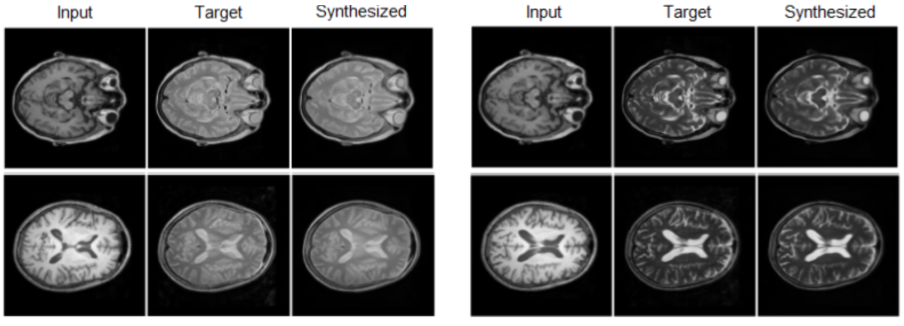
\includegraphics[width=\linewidth]{mri2mri.png}
  \center AI-synthesized images of proton density (left) or T2-weighted images from a T1-weighted image
\end{minipage}

\begin{minipage}[t]{\linewidth}
    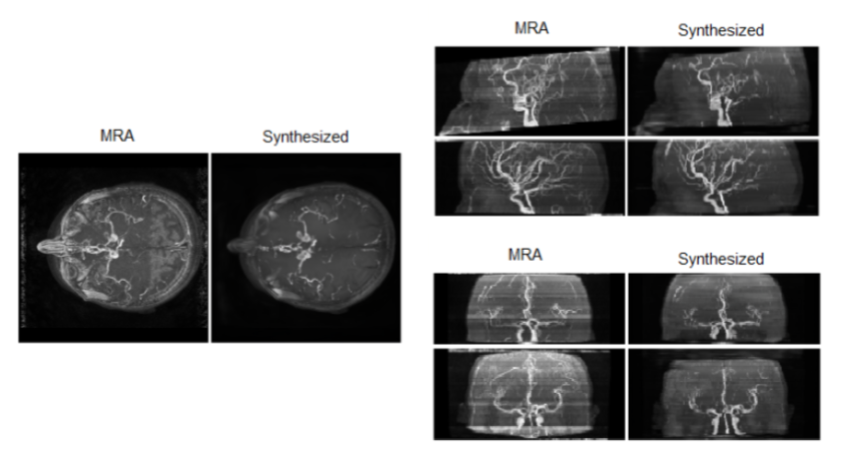
\includegraphics[width=\linewidth]{MRA.png}
    \center AI-synthesized MRA images from T1w + T2w + PD images.
\end{minipage}

\subsection*{Application: multi-modal image registration}

The algorithm was trained to synthesize T1w images from the DWI b=0 images. On a separate set of subjects, not used during training, we demonstrate that registration of T1w to DWI b=0 is more accurate using a synthesized T1w intermediary. This effect is shown here as mean absolute error (MAE; Figure 2) and is consistent both for the translation component (Mann Whitney U test, p $<$ 10e-7) and for rotation (Mann Whitney U test p $<$ 10e-4)

\begin{minipage}[t]{1.0\linewidth}
    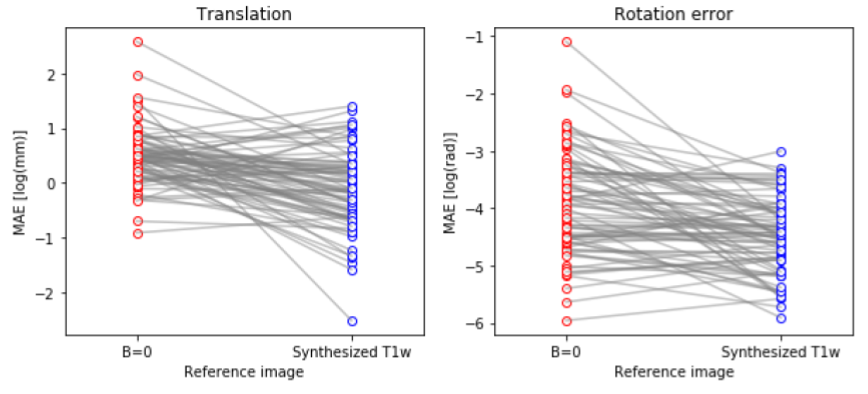
\includegraphics[width=\linewidth]{motion_correction.png}
\end{minipage}


%------------------------------------------------
\color{SaddleBrown} % SaddleBrown color for the conclusions to make them stand out

\section*{Conclusions}
\large
\begin{itemize}

\item \texttt{MRI2MRI} accurately transforms between brain MRI contrasts

\item This can be used to improve hard image processing tasks, such as cross-modal registration

\item Does this discover physical properties of the tissue?

\item Useful in other biomedical imaging data: OCTA, histology, ...

\end{itemize}

\color{DarkSlateGray} % Set the color back to DarkSlateGray for the rest of the content

%---------------------------------------------------------------------------	REFERENCES
%----------------------------------------------------------------------------

\nocite{*} % Print all references regardless of whether they were cited in the poster or not
\bibliographystyle{plain} % Plain referencing style
\footnotesize \bibliography{poster} % Use the example bibliography file sample.bib

%----------------------------------------------------------------------------%	ACKNOWLEDGEMENTS
%----------------------------------------------------------------------------
\subsection*{Acknowledgements} \footnotesize This research was supported through
a grant from the Gordon \& Betty Moore Foundation and the Alfred P. Sloan
Foundation to the University of Washington eScience Institute.


\includegraphics[height=2.6cm]{eSciencelogo.png}

\includegraphics[height=2.6cm]{SloanLogo.png}

\includegraphics[height=2.6cm]{MooreFdn.png}

%----------------------------------------------------------------------------

\end{multicols}
\end{document}
